% Henrik: Måske noget introducerende tekst til dette kapitel

\section{PACT analysis}\label{sec:PACT}
When designing an interactive system it is important to design it with the human in mind as the system is being developed for a specific purpose and context.
To do this the designers must explore the users who will eventually use the systems and for what purposes they are going to utilize it.
Depending on how well designers have implemented a way to convey their conception of a given system, different users will interpret it differently.
Their interpretation, being based on individual understanding and knowledge, regulates the users interactions with the system and thereby determines what it really does.
\citep{Benyon}
A model of this concept can be seen at \cref{fig:PACT-SystemImage}.

\begin{figure}[H]
	\centering
	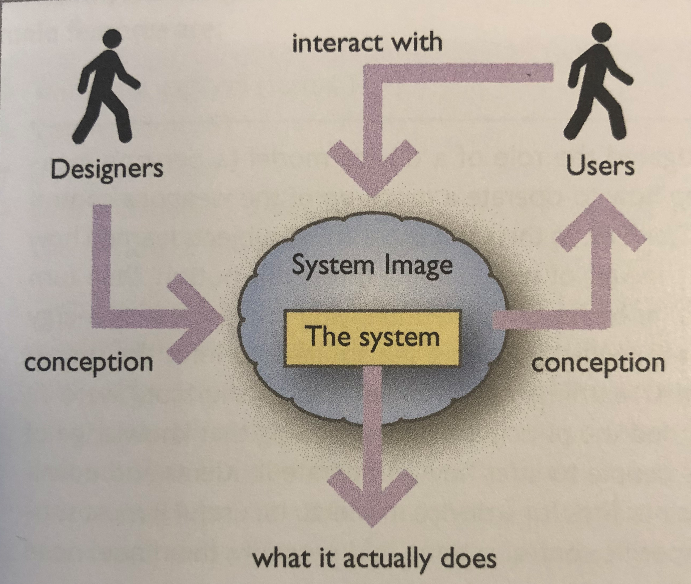
\includegraphics[width=0.4\textwidth]{billeder/SystemImage-Benyon.png}
	\caption{\textit{The System Image from \citep[p.~31]{Benyon}}}
	\label{fig:PACT-SystemImage}
\end{figure}

To help understand and reflect upon the users and their relation to an interactive system, the framework PACT is used.
PACT is an acronym for \textit{People, Activities, Context}, and \textit{Technology}.
This analysis framework is used to analyze the users, such that developers are able to design the system people-centered instead of machine-centered.
\citep{Benyon}
% Henrik: Er det nødvendigt at beskrive kort hvad "people-centered og machine-centered er?

The PACT theory presentation and analysis will be written congruently throughout this section. First the specific theory will be presented followed by the analysis.

\subsection{People}\label{PACT-people}
People differs from each others in many ways.
This element in the PACT analysis is a way to ponder upon these differences as well as a way to categorize the different users of a system.
Three differences usually discussed in this part of the analysis are \textit{physical, psychological}, and \textit{social}. \citep{Benyon}
% Henrik: Der er beskrevet hvad social og physical er - er det med vilje at der ikke er beskrevet hvad der menes med psychological er? :-)

Social differences is about how people use a system for different reasons and therefore can have various goals.
Additionally, there is also a big difference in people expertise levels which affects how an interface might be designed.
This is an important consideration since designing a system for a homogeneous group of people is  distinct from designing one for a heterogeneous group. \citep{Benyon}

Physical differences covers the relevant ways people differs in physical characteristics.
This could be, differences in perception from the five senses; sight, hearing, touch, smell and taste as well along with age, height or weight.
An example of a physical difference could be color blindness, which affects about $8\%$ of men and $0.5\%$ of women in the world \cite{ColourBlind}.
%\begin{example}
%As an example, when making an interface it is important to consider color blindness, since it affects about $8\%$ men and $0.5\%$ women in the world \cite{ColourBlind}.
%\end{example}

In the case described in this report, see \cref{sec:CaseDescription}, there are four main groups of people that needs to be considered.
These are the quality manager, secretaries, department heads, and everyday workers.
This is a heterogeneous group with different levels of IT experience ranging from no skills with IT and therefore cautious about it, to the level of everyday office work.
The group also has different levels of domain expertise ranging from novice to expert which needs to be considered.
The quality manager is a domain expert and therefore has different needs of the system than the everyday worker with no expertise.
% Taniya: quality chief or quality manager?
% 	Henrik: Jeg har ændret det til quality manager
% Henrik: Det er vel en antagelse, at "everyday worker with no expertise"?

Furthermore, issues such as colorblindness, other eye handicap as well as bad memory needs to be considered when designing the system and interface.

\subsection{Activities}\label{PACT-actvities}
When considering the activities developers or designers should focus on the overall purpose of these.
When that's completed the main features can be considered such as described below:

When considering the people using the system, which is explored under \cref{sec:PACT-people}, there are two different activities in relation with the system.
There is the activities of the secretaries and those of the everyday workers perspectives.
The secretary and quality manager has a more administrative role.
%, where the secretary in part writes and maintains the handbook.
The overall activities for this role is to manage, update and access a handbook mostly the newest version but also possibly older versions as well.
It is necessary to uphold standards set by the government to retain the companies certifications.
Whereas the workers ''only'' has to read certain documents.

\textit{Temporal aspects} covers different features in the system as well as a consideration of how the users interaction with the system is done during a day.
Starting with the considerations of users interactions, one need to consider among other:

\begin{itemize}
	\item How often is the interactive system used?
	\item Is the interactions with the system done continuously or interrupted?
\end{itemize}

For the temporal aspects in a given system the developers need to consider things such as; time pressures, peaks and, and the response time of a given activity. \citep{Benyon}

When doing the activities users may experience interruptions and the system should therefore be simple to use and easy to get back to.
Being easy to use is a feature most relevant for the everyday workers, as they only occasionally need to read documents and therefore is less in contact with the system.
This makes it necessary to make the system as easily accessible for them as possible.
The activities would most often be done during business hours, from 8-16 on weekdays, though may be accessed outside of this time frame as well.

% Taniya: kunne måske være en ide at kort nævne administrator at selvom de bliver forstyrret med notifikationer fra systemetm så skal admin hurtigt kunne vende tilbage til arbejdsopgaven admin var i gang med. Men stadig nemt kunne se/huske/ finde tilbage til de notifikationer, så de hellere ikke bliver glemt.

\textit{Cooperation} is simply the consideration of whether or not the activity is done in cooperation with others, alone, or a mix hereof, as well as how and when a possible cooperation is needed.
This is an important consideration since a system which is done in cooperation with others needs to have an awareness of all the users, be able to coordinate it between these and maybe have a communication system implemented as well.
On the other hand if the activities is done completely alone these features are not necessary. \citep{Benyon}

The cooperation aspect is mostly relevant for the quality manager and secretary as they are maintaining the handbook documents.
Here it is necessary to not only write new versions of a document but also make sure that the newest versions are approved.
Though writing the documents in itself does not require collaboration.
As for the worker's activities, there is no cooperation involved as all the workers need to read the newest, relevant documents individually.

% Taniya: The cooperation aspect also involves the approvers?

\textit{Complexity} describes the question of how well-defined the activity is.
Is it a well-defined task which can be done in a simple step-by-step design,
Or is it a vague task, which would need users to browse around? \citep{Benyon}

In this project, the activities are quite well-defined overall.
For the administrative personnel it is well-defined that whenever a new document has been written, it is imperative that it is approved and then inserted.
Here the oldest, and now outdated, document is being archived and stored for a set period of time.
The secretary needs to make sure that the affected everyday workers read and understand the new documents.

% Taniya: er det sekretær der sørger for at dokumenter bliver læst? er det ikke afdelingsleder?

\textit{Safety Critical} has two sides to it.
First is whether or not the activity in itself is ``safety-critical'' where mistakes could be reason for injury or serious accidents.
Second is the consideration of ``what will happen when mistakes and errors are made?'' which is important for any developer to reflect upon and then design for these circumstances.
\citep{Benyon}

There are no physical safety issues to consider in relation to the system, though there are serious consequences to consider if the handbook documents do not live up to regulations.
It is required that there are updated handbook documents and that the archived versions of these documents are stored somewhere.
If this is not upheld then the firm could suffer loss of certification, which would result in great loss of revenue.
%Taniya: tænker at der mangler en kilde? der er vel også nogle lovpligtige standarder/regler der skal overholdes ellers får virksomheden en bøde?
% Henrik: Måske bare henvis til det der er skrevet om ISO/Standarder?

\textit{The nature of the content} is a more technical reflection of which data requirements are needed for the activity as well as what media it requires.
\citep{Benyon}

It is important that the system is able to handle Microsoft documents such as Word and Excel as these are the filetypes used to write the documents.
Furthermore the system should support large quantities of these files as the archived versions of the documents are usually stored for three to five years.

\subsection{Contexts}
Activities always occur in a context which will be explored in this section.
Context can be thought of, as something that surrounds activities as well as a feature which binds them together into a whole.
Usually when considering this point in PACT the three points: \textit{Physical environment, Social context}, and \textit{Organizational context} are at the main focus.
\citep{Benyon}

The physical environment might cover everything from weather to geographical placement of where the activity is done.
It is an analysis of the surrounding environment which may have effect on how users perform activities.
\citep{Benyon}

In relation to the people in this case there are two main physical contexts to consider.
For the quality manager and secretary an office context is most likely as they handle administrative work.
For the everyday workers the context could differ dramatically as their functions may differ from each other.
The main focus here should be that the handbook documents should be easily accessible, no matter in which context the workers are located.
Previous to the implementation of this project, the most common way that the handbooks were used by employees were in printed out form, which allowed the use of the documents in circumstances not conductive to electronic equipment. %Or rather, too conductive. Get it?

%Social context covers things such as whether or not the environment is supportive, or the user is alone in using and learning the activities.
%It is also an reflection on if the social norms may dictate certain designs.

% Taniya: så vi nævner ikke social context ?

The organizational context is among other an examination of the impact new technology may have on the organization.
It is also a review of the circumstances under which the activities is done; time, place and so on.
\citep{Benyon}

% Taniya: The organizational context er ikke beskrevet ift. projektets sammenhæng?

The technological aspect is presumably most relevant for the secretary and the quality manager as they will be doing most of the work in the handbook.
Both of them would be working on a regular computer which utilizes the Windows operating system. % Henrik: Har fjernet "or Mac OS-system."
%Anna: Hvad tænker folk hænger de to afsnit ovenfor sammen?, giver det mening at afsnittet ovenfor er en organizational context?
%Taniya: nej, det synes jeg ikke :( forventede at læse om Physical environment, Social context, Organizational context. Føler lidt at The technological aspect kom ud af det blå

\subsection{Technologies}
Technologies is the reflection on the medium which interactive system designers work with.
It covers looking into elements such as what medias and technologies is needed to best get input and present the output, and review the communication between the needed devices.
Furthermore, it also examines the content, which concerns the data in the system and its form.
Good content is defined as accurate, up to date, relevant and well presented.
\citep{Benyon}

Since the activities are most often done in an office environment, on a standard PC, the input medias are keyboard and mouse.
In addition output is presented through a monitor, or for the workers on the factory floor through a printed version of the handbook, or parts of it.
The contents on the monitor are presented through a Graphical User Interface (GUI).
Furthermore, the communication user-to-user is usually done through telephone, while it between devices are done over a Network, such as the internet.
Lastly, is the communication from the system to a user done through notifications.
% Taniya: notification som email, sms? snakker vi om hvordan det er nu ? eller snakker vi om systemet vi har tænkt os at lave til dem?

% Det er meget svingende om der er snakke om "secretary" eller "secretaries" igennem hele PACT :-)
